{\centering \nonumsubsection{B \hspace{1em} 组}}
\begin{xiaotis}
\setcounter{cntxiaoti}{15}
\begin{enhancedline}

\xiaoti{求证:过一点和一条直线垂直的所有直线都在一个平面内。}

\xiaoti{在 $120^\circ$ 角的二面角 $\alpha{-}a{-}\beta$ 中,$A \in \alpha$,$B \in \beta$。
    已知点 $A$ 和 $B$ 到棱 $a$ 的距离分别为 2 和 4,且 $AB = 10$。
    求直线 $AB$ 和棱 $a$ 所成的角及直线 $AB$ 和平面 $\beta$ 所成的角。
}

\xiaoti{空中有一气球,它和地面的距离是 $h$。在气球的东南 $A$ 处看气球时,仰角是 $\theta_1$;
    同时在气球的西南 $B$ 处看气球时,仰角是 $\theta_2$。 $A$、$B$ 两地的距离是 $a$。求证:
    $$ h = \dfrac{a}{\sqrt{\cot^2\theta_1 + \cot^2\theta_2}} \juhao $$
}

\xiaoti{将半径为 $R$ 的四个球,两两相切地放在桌面上。求上面一个球的球心到桌面的距离。}

\xiaoti{要从半径为 210 cm 的圆形铁皮上剪下一些扇环做成漏斗。漏斗一端的直径是 40 cm,
    另一端直径是 140 cm,母线长 150 cm。计算这块铁皮能做几个漏斗,怎样剪法?
}

\xiaoti{测定某些材料的硬度,可用标准钢球(直径 10 mm)放在材料上,加上一定的压力 $P$ kg,
    将材料表面压成球冠形凹痕。设凹痕的面积是 $S\;\pfhm$,这时材料的硬度是 $P/S \;\text{kg/mm}^2$。
    如果所加压力是 $3.0 \times 10^3$ kg,凹痕直径是 4.1 mm,计算这材料的硬度。
}

\xiaoti{如图,将正方体的棱分为 4 等分,在 $\exdfrac{1}{4}$ 处截去各棱角得到一个多面体。
    正方体体积减少几分之几(不证)?
}

\begin{figure}[htbp]
    \centering
    \begin{minipage}[b]{7cm}
        \centering
        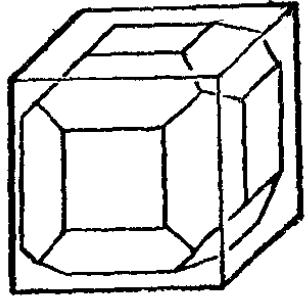
\includegraphics[width=4cm]{../pic/ltjh-zongfuxi-22.png}
        \caption*{(第 22 题)}
    \end{minipage}
    \qquad
    \begin{minipage}[b]{7cm}
        \centering
        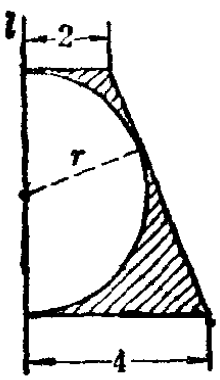
\includegraphics[width=3cm]{../pic/ltjh-zongfuxi-23.png}
        \caption*{(第 23 题)}
    \end{minipage}
\end{figure}

\xiaoti{求图中阴影部分绕轴 $l$ 旋转所成旋转体的全面积和体积。}

\xiaoti{一个圆锥侧面的母线和底面直径相等(等边圆锥),有一内切球。
    已知圆锥底面直径为 $2r$,求球的体积。
}

\begin{withstar}

\xiaoti{下图是正十二面体、正二十面体的表面去掉一个面后,连续变形所成的平面图形。
    数出它们的顶点数 $V$、棱数 $E$ 及面数 $F$ 来验证 $V + F - E = 1$。
}

\begin{figure}[htbp]
    \centering
    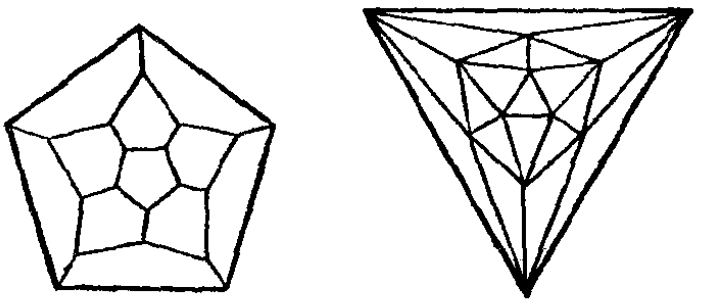
\includegraphics[width=9cm]{../pic/ltjh-zongfuxi-25.png}
    \caption*{(第 25 题)}
\end{figure}

\xiaoti{求证:如果简单多面体的所有面都是奇数边的多边形,那么面数是偶数。}

\end{withstar}
\end{enhancedline}
\end{xiaotis}
